\documentclass[12pt]{article}
\usepackage[spanish, english, es-tabla]{babel}
\usepackage[utf8]{inputenc}
\usepackage[left = 2cm, right = 2cm, bottom = 2cm, top = 3cm]{geometry}
\usepackage{amsmath, amssymb}
\usepackage{graphicx}
\usepackage{hyperref}
\usepackage{listings}
\usepackage{courier}

\usepackage[dvipsnames]{xcolor}

\renewcommand{\lstlistingname}{Listado}
\renewcommand{\lstlistlistingname}{Listado de códigos}

% https://tex.stackexchange.com/questions/60209/how-to-add-an-extra-level-of-sections-with-headings-below-subsubsection
\newcommand{\subsubsubsection}[1]{\paragraph{#1}\mbox{}\\}
\setcounter{secnumdepth}{4}
\setcounter{tocdepth}{4}

\begin{document}
	\selectlanguage{spanish}
	
	%%%% PORTADA
	\title{\textbf{Aplicación de técnicas de virtualización ligera para la evaluación de redes de comunicaciones} \\ 
	\addvspace{10px} \large \textit{Trabajo Final de Estudios} \\
	\large Ingeniería Telemática}
	\author{Autor: Enrique Fernández Sánchez \\ Tutor: Josemaria Malgosa Sanahuja \\ \\Universidad Politécnica de Cartagena}
	
	%% EDITAR PARA SEGUIMIENTO DE VERSIONES
	\date{Revisión Septiembre 2021}
	
	\maketitle
	
	%%% END PORTADA
	
	\pagebreak
	
	\tableofcontents
	
	\pagebreak
	
	\addcontentsline{toc}{section}{Índice de figuras}
	\listoffigures
	\addcontentsline{toc}{section}{Índice de tablas}
	\listoftables
	\addcontentsline{toc}{section}{Listado de códigos}
	\lstlistoflistings
	
	\pagebreak
	
	%%% Glosario
	\pagebreak
	\section*{Glosario de términos}
	\addcontentsline{toc}{section}{Glosario de términos}
	
	\noindent{\large \textbf{NFV} (\textit{Network Function Virtualization})}. \textit{Network Function Virtualization}, o bien, Virtualización de funciones de red.\\
		 
	\noindent{\large \textbf{Namespace}}. \textit{Espacio de nombres}\\
		 
	\noindent{\large \textbf{NS} (\textit{Network namespace})}. Tipo de espacio de nombres en Linux que tiene por función aislar la parte de red de la máquina host.\\
	
	\noindent{\large \textbf{Linux}}. Sistema operativo tipo UNIX, de codigo abierto, multiplataforma, multiusuario y multitarea.\\
		 
	\noindent{\large \textbf{Kernel de Linux}}. Núcleo del sistema operativo Linux.\\
		 
	\noindent{\large \textbf{PID} (\textit{Process Identifier})}. Identificador de procesos que están ejecutándose bajo un sistema tipo Linux.\\
	
	\noindent{\large \textbf{UID} (\textit{User identifier})}. Encontrado normalmente como un número o palabra, supone un identificador de usuario dentro del sistema Linux.\\
	
	\noindent{\large \textbf{GID} (\textit{Group Identifier})}. Al igual que sucede con el UID, suele aparecer como un número o palabra y hace referencia al identificador de grupo dentro del sistema de Linux.\\
		 
	\noindent{\large \textbf{root}}. Cuenta superusuario del sistema operativo Linux.\\
		 
	\noindent{\large \textbf{veth-pair} (\textit{Virtual Ethernet Pair})}. Tipo de interfaz virtual. Funcionan de dos en parejas.\\
		 
	
	\pagebreak
	
	%%% TODO
	\section*{Agradecimientos}
	\addcontentsline{toc}{section}{Agradecimientos}
	
	\pagebreak
	
	%%% TODO
	\section{Introducción}
	\noindent Con el fin de concluir los estudios de grado en ingeniería telemática, es necesaria la investigación y el posterior desarrollo del \textit{Trabajo Fin de Estudios} (TFE). Dicho trabajo, tiene como objetivo enfrentar al alumno a un proceso de investigación en el que pueda aplicar los conceptos que ha ido aprendiendo durante su paso por el grado, además pudiendo añadir puntos de innovación, y aportar soluciones nuevas a un proyecto en específico.\\
	
	\noindent En este documento, recojo lo que sería mi memoria en relación al TFE. En dicho documento detallaremos las diferentes investigaciones realizadas sobre el concepto de virtualización en sistemas Linux, como funcionan los contenedores y como utilizar la virtualización ligera para la evaluación de redes de comunicaciones, en nuestro caso, de conmutación de paquetes.
	
	\subsection{Contexto del trabajo}
	\noindent Este proyecto nace con el objetivo de profundizar en conceptos novedosos para el ámbito de red, como por ejemplo podría ser NFV. Definimos NFV (Network Function Virtualization) como la virtualización de hardware físico de red, con el fin de solucionar problemas de escalabilidad y de optimización.\\
	
	 \noindent Además, trabajaremos sobre otras tecnologías igual de importantes como pueden ser la virtualización de recursos, o los bien conocidos \textit{contenedores}. Particularizaremos estas tecnologías y las acercamos al campo de conocimiento de la telemática para utilizarlas con el fin de evaluar y simular redes de conmutación de tipo IP. \\
	
	\noindent Partiendo de supuesto de que las herramientas más sencillas de simulación de redes se nos pueden quedar cortas en cuanto queremos escalar el sistema, nos topamos en que otras soluciones pueden ser mucho más \textit{resource hungry} de lo que podríamos imaginar. Además, tampoco podemos contar con realizar dichas pruebas de manera física, ya que el presupuesto del proyecto escalaría de nivel exponencial. Esto sucede ya que deberíamos configurar cada dispositivo de manera específica, y después proceder a interconectarlos con una tecnología de red adecuada, que en nuestro caso, son tecnologías en fase de desarrollo o evaluación de prestaciones.\\
	
	\noindent Conociendo las limitaciones, establecemos una serie de objetivos de cara a evaluar el viaje que realicemos durante ese proyecto, y poder evaluar posteriormente los avances que hemos podido conseguir, y además las conclusiones vinculadas a estos. Estos objetivos podrían ser:\\
	\begin{itemize}
		\item Análisis de diferentes opciones de simulación de redes. Tanto basadas en virtualización, como las que no.
		\item Comprender la diferencia entre virtualización \textit{ligera} y virtualización \textit{dura}.
		\item Profundizar en el concepto de \textit{interfaces virtuales} en Linux.
		\item Definir que es el \textit{espacio de nombres} y ejemplificar cada uno de ellos.
		\item Aproximación al concepto de contenedor, relacionarlo con los \textit{espacio de nombres}.
		\item Aportar una solución válida para la simulación y evaluación de un sistema, utilizando la virtualización ligera.
	\end{itemize}
	
	%\pagebreak
	
	%%% TODO
	\subsection{Objetivos}
	\noindent Como bien hemos adelantado en el apartado anterior, el objetivo principal de este proyecto es el de analizar la situación en el ámbito de simulación y evaluación de redes de comunicación, además, concretar en aquellas soluciones que estén basadas en virtualización ligera. Por lo tanto, se pretende: \\
	\begin{itemize}
		\item Aprendes los conceptos básicos de la virtualización de sistemas de red (NFV).
		\item Estudiar, dentro del sistema operativo Linux, las diferentes tecnologías que nos permiten adoptar soluciones NFV.
		\item Definir que es \textit{espacio de nombres} y como podemos aplicarlo para virtualizar redes.
		\item Desgranar el concepto amplio de contenedor.
		\item Desarrollar una aplicación conceptual para la evaluación de un sistema en concreto, utilizando virtualización ligera.
	\end{itemize}

	\subsection{Descripción de los capítulos restantes de la memoria}
	\noindent En este apartado se comentará brevemente la distribución de capítulos de la memoria. Además, se mencionará que temas se han abordado en cada uno de ellos.
	\begin{itemize}
		\item \textbf{Capítulo 1}: Introducción.
		\item \textbf{Capítulo 2}: Virtualización de funciones de red.
		\item \textbf{Capítulo 3}: Interfaces de red virtuales en Linux.
		\item \textbf{Capítulo 4}: Espacio de nombres en Linux.
		\item \textbf{Capítulo 5}: Virtualización.
		\item \textbf{Capítulo 6}: Caso práctico: Virtualización para la simulación de redes.
		\item \textbf{Capítulo 7}: Conclusiones.
	\end{itemize}
	
	
	\pagebreak
	
	\section{Virtualización de funciones de red}
	%% https://www.youtube.com/watch?v=3JEAK66wujg
	\noindent NFV surge a partir de las necesidades de las operadoras para solucionar problemas de gran escala de la red. Este movimiento nace en X. Uno de los objetivos que se pretenden desde el punto de vista de las operadoras, es reducir los costes y optimizar la red. Esto sucede ya que las redes actuales sufren de tres problemas: falta de escalabilidad en momentos precisos y específicos; excasa flexibilidad de la red, en momento específicos necesitaremos modificar funcionamientos de nodos en concreto, pero no se nos posibilita; falta de innovación en la gestión de los recursos, nuevos servicios, etc. Todo esto ocurre ya que las redes de las operadoras han evolucionado muy poco. \\
	
	\noindent La solución que se propone para estos problemas es la virtualización de las redes. Esta corriente nace en octubre de 2012, a partir del \textit{paper} [\ref{paper nfv 2012}], creado con la colaboración de 13 operadoras de red internacionales. En el, se plantea el objetivo de esbozar los diferentes beneficios y retos de la virtualización de recursos de red, y los motivos para fomentar una colaboración internacional para acelerar el desarrollo y el despliegue de soluciones interoperables basadas en servidores estándar del sector de gran volumen. Esto supone el primer paso a la nueva tecnología de las redes. \\
	
	\noindent La virtualización de las redes consiste en el desarrollo de un enfoque en software de las redes. Intenta solucionar los problemas planteados, aportando innovación y una mayor escalabilidad de las redes. Supone el conjunto de SDN y NFV, normalmente la virtualización de redes no existe una sin la otra [\ref{youtube: nfv y sdn cristina}].\\
	
	\begin{figure}[h]
		\begin{center}
			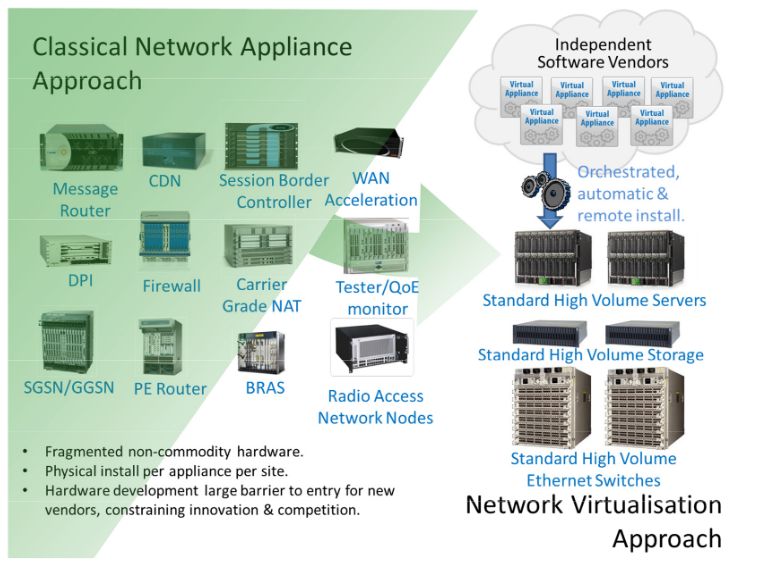
\includegraphics[width=0.7\textwidth]{img/classic_network_vs_nfv.png}
			\label{imagen comparativa classic network nfv}
			\caption{Comparativa enfoque clásico de las redes contra el enfoque virtualizado. [\ref{paper nfv 2012}]}
		\end{center}
	\end{figure}

	\pagebreak
	
	\noindent La actualidad es cada dispositivo, corresponde con un aparato físico. Son aparatos embebidos y solo cumplen una función específica. Utilizando la virtualización de red, podemos llegar al punto de tenerlo todo virtualizado. Tenemos una 'imagen' de router que la podemos desplegar en cualquier ordenador de caracter general, y cumplir diferentes funciones a la vez (que un router sea a la vez un firewall, por ejemplo).\\
	
	\noindent Las funciones de red están basadas en tener un software y hardware específico para cada dispositivo. NFV nos aporta que esos recursos software y hardware, se despliegan en servidores físicos de proposito general. Por lo tanto, un mismo nodo físico, puede ser DHCP, router o Firewall.\\
	
	%% IMAGEN
	
	
	
	
	
	
	\noindent Entendemos la virtualización ligera como un tipo de virtualización de un sistema. Dicha virtualización se hace a nivel de sistema operativo, aportando que existan diferentes espacios de usuarios aislados entre sí, y todo esto estando todos bajo el mismo kernel. Las diferentes implementaciones de 
	
	\pagebreak
	
	\section{Interfaces de red virtuales en \textit{Linux}}
	\noindent En este capítulo, vamos a profundizar en el concepto de interfaces de red virtuales, pero las específicas al sistema operativo basados en el kernel de Linux. Hacemos esto ya que los servidores utilizados a gran escala, la mayoría hacen uso de distribuciones de Linux
	
	
	\noindent Linux dispone de una selección muy diferente de interfaces de red que nos permiten, de manera sencilla, el uso de máquinas virtuales o contenedores. En este apartado vamos a mencionar las interfaces más relevantes de cara a la virtualización ligera que proponemos para el despliegue de una red virtualizada. Para obtener una lista completa de las interfaces disponibles, podemos ejecutar el siguiente comando \texttt{ip link help}.\\
	
	\par \noindent En este trabajo, vamos a comentar la siguientes interfaces:
	\begin{itemize}
		\item eth0:\{0,1,2...\}
		\item eth0.\{0,1,2...\} VLAN
		\item eth0.\{0,1,2...\} VLAN 802.1ad
		\item VETH pairs
		\item TUN/TAP
	\end{itemize}


	\subsection{Nombres predecibles interfaces de red. \texttt{systemd networkd v197}}
	 \noindent Para la explicación de las diferentes interfaces, vamos a suponer que estamos utilizando el nombrado de interfaces de red antiguo. Esto proviene de que en la últimas versiones del kernel, se ha cambiado la forma en la que las interfaces de red son nombradas por Linux. Es por esto por lo que antes podíamos tener interfaces tal que \texttt{eth0} y ahora nos encontramos con la siguiente nomenclatura \texttt{enps30}. Este cambio surge ya que anteriormente se nombraban las diferentes interfaces conforme el propio ordenador estaba en la etapa de \texttt{boot}, por lo que podría pasar que a lo que nosotros entendíamos como \texttt{eth1}, en el próximo arranque fuera \texttt{eth0}, dando lugar a incontables errores en el sistema. Es por esto por lo que se empecó a trabajar en soluciones alternativas. Por ejemplo, la que hemos utilizado de ejemplo, utiliza la información aportada por la BIOS del dispositivo para catalogarlo en diferentes categorías, con su formato de nombre para cada categorías. Dichas clasificación corresponde con las siguientes:
	\begin{enumerate}
		\item Nombres incorporando Firmware/BIOS que proporcionan un número asociado a dispositivos en la placa base. (ejemplo: \texttt{eno1})
		\item Nombres incorporando Firmware/BIOS proveniente de una conexión PCI Express hotplug, con número asociado al conector. (ejemplo: \texttt{ens1})
		\item Nombres que incorporan una localización física de un conector hardware. (ejemplo: \texttt{enp2s0})
		\item Nombres que incorporan una la MAC de una interfaz. (ejemplo: \texttt{enx78e7d1ea46da})
		\item Sistema clásico e impredecible, asignación de nombres nativa del kernel. (ejemplo: \texttt{eth0})
	\end{enumerate}
	
	\pagebreak
	\subsection{\texttt{enp2s0:\{0,1,2...\}}}
	\par \noindent Todas las interfaces asociadas comparten la misma dirección MAC. Cada una de ellas, recibe el nombre de \textit{aliases}. La funcionalidad principal que tienen este tipo de interfaces es la de asignar varias direcciones de IP a una misma interfaz de red.
	
	\begin{verbatim}
$ ip addr add 192.168.56.151/24 broadcast 192.168.56.255 dev enp2s0 
label enp2s0:1
	\end{verbatim}

	\par \noindent Sin embargo, el comando \texttt{iproute2} admite esta misma funcionalidad sin tener que crear interfaces de red extra. Para ello, solo tenemos que asociar cada IP con la interfaz de red deseada.
	\begin{verbatim}
$ ip addr add 192.168.56.151/24 dev enp2s0
$ ip addr add 192.168.56.251/24 dev enp2s0
	\end{verbatim}

	\subsection{VLAN. \texttt{enp2s0.\{0,1,2...\}}}
	\par \noindent Mismo concepto que la interfaz anterior, sin embargo, utilizamos el estandar 802.1q, que permite etiquetar las tramas, para crear una red lógica independiente. Es necesario que la interfaz a la que estemos asignando, sea un puerto trunk, o bien sea tagged para una VLAN específica.
	
	\begin{verbatim}
$ ip link add link enp2s0 name enp2s0.{num} type vlan id {num}
$ ip addr add 192.168.100.1/24 brd 192.168.100.255 dev enp2s0.{num}
$ ip link set dev enp2s0.{num} up
	\end{verbatim}

	\begin{figure}[h]
		\begin{center}
			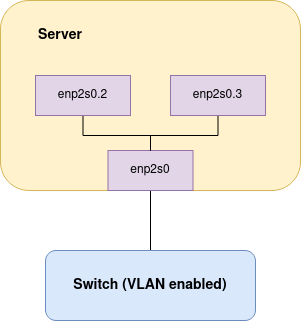
\includegraphics[width=0.4\textwidth]{img/diag_vlan.png}
			\caption{Diagrama conexión VLANs}
		\end{center}
	\end{figure}

	\pagebreak
	
	\subsection{VLAN 802.1ad. \texttt{enp2s0}.\{0,1,2...\}}
	
	\subsection{Pares VETH.}
	\noindent Los VETH (Ethernet virtuales) son un dispositivo que forman un túnel local ethernet. El dispositivo se crea en parejas.\\
	
	\noindent Los paquetes transmitidos por un extremo del VETH se reciben inmediatamente en el otro extremo. Si alguno de ellos se encuentra apagado, decimos que el link de la pareja esta también apagado.\\
	
	\begin{figure}[h]
		\begin{center}
			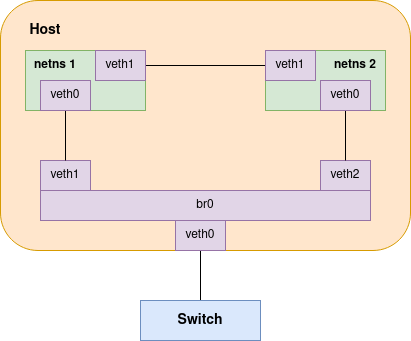
\includegraphics[width=0.5\textwidth]{img/VETH.png}
			\caption{Diagrama VETH y netns}
		\end{center}
	\end{figure}

	\noindent Es necesario utilizar VETH cuando un namespace necesita comunicarse con el host, o viceversa.\\
	
	\noindent La configuración que tenemos que realizar para tener el diagrama de la Figura 2.
	
	\begin{verbatim}
$ ip netns add net1
$ ip netns add net2
$ ip link add veth1 netns net1 type veth peer name veth1 netns net2
	\end{verbatim}

	\noindent De esta manera, tendríamos creados los namespaces \texttt{net1} y \texttt{net2}, que estarían interconectados con las interfaces \texttt{veth1} y \texttt{veth2}. Nos quedaría asignar una IP a cada interfaz. 
	
	
	%% https://blog.scottlowe.org/2013/09/04/introducing-linux-network-namespaces/
	\begin{verbatim}
$ ip netns exec net1 ip addr add 10.1.1.1/24 dev veth1
$ ip netns exec net1 ip link set veth1 up
$ ip netns exec net2 ip addr add 10.1.1.2/24 dev veth1
$ ip netns exec net2 ip link set veth1 up
	\end{verbatim}

	%% https://www.eduardocollado.com/2018/09/25/podcast-176-primeros-pasos-con-open-vswitch/
	
	\noindent Ahora nos quedaría la parte de crear un bridge entre las diferentes interfaces virtuales que hemos creado. Para esto, podemos utilizar una interfaz tipo \textit{bridge} de Linux, o bien podemos configurar un \textit{bridge} usando \textit{Open VSwitch}.
	
	%% https://matthewarcus.wordpress.com/2018/02/04/veth-devices-network-namespaces-and-open-vswitch/
	
	\begin{verbatim}
$ ip link add veth1_br type veth peer name veth0 netns net1
$ ip link add veth2_br type veth peer name veth0 netns net2
$ ovs-vsctl add-br ovsbr0
$ ovs-vsctl add-port ovsbr0 veth1_br
$ ovs-vsctl add-port ovsbr0 veth2_br
$ ovs-vsctl add-port ovsbr0 <outbound interface>
	\end{verbatim}

	\noindent Añadimos las direcciones IP que nos faltan:
	
	\begin{verbatim}
$ ip addr add 10.1.1.10/24 dev veth1_br
$ ip link set veth1_br up
$ ip addr add 10.1.1.20/24 dev veth2_br
$ ip link set veth2_br up
$ ip netns exec net1 ip addr add 10.1.1.15/24 dev veth0
$ ip netns exec net1 ip link set veth0 up
$ ip netns exec net2 ip addr add 10.1.1.25/24 dev veth0
$ ip netns exec net2 ip link set veth0 up
$ ip netns exec net1 ip link set lo up
$ ip netns exec net2 ip link set lo up
	\end{verbatim}

	\subsection{TUN/TAP}
	\noindent Permite conectar una aplicación en específico con el kernel, utilizando un dispositivo Ethernet. Una aplicación puede acceder al tuntap o bien crearlo ella misma. \\
	
	\noindent TUN trabaja a nivel IP (capa 3), tiene por función principal definir túneles. No entiende nada de ARP (ni nada de nivel 2).\\
	
	\noindent TAP trabaja solo a nivel de MAC (entiende ARP, etc.) y sirve directamente para un bridge virtual. Los túneles los puede crear directamente el comando ip, por lo que la interfaz TUN apenas se utiliza. Sin embargo, TAP es muy utilizado para crear un \textit{bridge}.\\
	
	\noindent Un \textit{bridge} puede incorporar interfaces TAP. En este caso, la aplicación que lo monitoriza puede ser un hipervisor (Virtualbox, Qemu, libvirt), es decir, el \textit{bridge} está dentro del kernel.
	
	\noindent 
	
	\pagebreak
	
	
	
	\pagebreak
	\section{Espacio de nombres en \textit{Linux}}
	\subsection{¿Qué es un \textit{espacio de nombres}?}
	\noindent Los \textit{espacios de nombres}, o también llamados, \textit{namespaces}, son una característica del kernel de Linux que permite gestionar los recursos del kernel, pudiendo limitarlos a un proceso o grupo de procesos. Suponen una base de tecnología que aparece en las técnicas de virtualización más modernas (como puede ser Docker, Kubernetes, etc). A un nivel alto, permiten aislar procesos respecto al resto del kernel. \\
	
	\par \noindent El objetivo de cada \textit{namespaces} es adquirir una característica global del sistema como una abstracción que haga parecer a los procesos de dentro del \textit{namespace} que tienen su propia instancia aislada del recurso global.
	
	\subsection{¿Cúantos \textit{namespaces} hay?}
	\par\noindent El kernel ha estado en contaste evolución desde que 1991, cuando Linus Torvalds comenzó el proyecto, actualmente sigue muy activo y se siguen añadiendo nuevas características. El origen de los namespaces se remonta a la versión del kernel 2.4.19, lanzada en 2002. Conforme fueron pasando los años, más tipos diferentes de namespaces se fueron añadiendo a Linux. El concepto de \textit{User namespaces}, se consideró terminado con la versión 3.9.\\
	\par \noindent Actualmente, tenemos 8 tipos diferentes de namespaces, siendo el último añadido en la versión 5.8 (lanzada el 2 de Agosto de 2020). 
	
	\begin{enumerate}
		\item UTS (hostname)
		\item Mount (mnt)
		\item Process ID (pid)
		\item Network (net)
		\item User ID (user) 
		\item Interprocess Communication (ipc)
		\item Control group (cgroup)
		\item Time
	\end{enumerate}
	
	\pagebreak
	
	\subsubsection{UTS namespace}
	\par \noindent El tipo más sencillo de todos los namespaces. La funcionalidad consiste en controlar el hostname asociado del ordenador, en este caso, del proceso o procesos asignados al namespace. Existen tres diferentes rutinas que nos permiten obtener y modifcar el hostname: 
	\begin{itemize}
		\item \textit{sethostname()}
		\item \textit{setdomainname()}
		\item \textit{uname()}
	\end{itemize}
	En una situación normal sin namespaces, se modificaría una String global, sin embargo, si estamos dentro de un namespace, los procesos asociados tienen su propia variable global asignada.\\
	
	% example uts: https://medium.com/@teddyking/linux-namespaces-850489d3ccf
	% https://www.cloudsavvyit.com/742/what-are-linux-namespaces-and-what-are-they-used-for/
	\par \noindent Un ejemplo muy basico de uso de este namespaces podría ser el siguiente:\\
	\begin{lstlisting}[language=bash, caption=Example usage UTS namespace]
$ sudo su			# super user
$ hostname			# current hostname
> arch-linux					
$ unshare -u /bin/sh		# shell with UTS namespace
$ hostname new-hostname		# set hostname
$ hostname			# check hostname of the shell
> new-hostname
$ exit				# exit shell and namespace
$ hostname			# original hostname
> arch-linux
	\end{lstlisting}

	\addvspace{10px}

	\par \noindent En el ejemplo planteado, vemos que utilizamos el comando \texttt{unshare}. Utilizando la documentación de dicho comando, \texttt{man unshare}. Podemos deducir los siguiente:
	\begin{itemize}
		\item Ejecuta un programa con algunos namespaces diferentes del host.
		\item En los parametros podemos especificar cual o cuales namespaces queremos desvincular.
		\item Tenemos que especificar la ruta del ejecutable que queremos aislar
		\item La sintaxis sería tal que: \texttt{unshare [options] <program> [<argument>...]}
	\end{itemize}
	
	\pagebreak
	
	\subsubsection{Mount namespace}
	\par \noindent Un \textit{mount namespace (mnt)} supone otro tipo de espacio de nombres, en este caso relacionado con los \textit{mounts} de nuestro sistema. Lo primero es entender a que nos referimos cuando hablamos de \textit{mount}. \textit{Mount}, o montaje, hace referencia a conectar un sistema de archivos adicional que sea accesible para el sistema de archivos actual de un ordenador. Un \text{mount}, tiene asignado lo que se llama \textit{mount point}, que corresponde con el directorio en el que está accesible el sistema de archivo que previamente hemos montado.\\
	
	\par \noindent Por lo tanto, un namespace de tipo \textit{mount} nos permite modificar un sistema de archivos en concreto, sin que el host pueda ver y/o acceder a dicho sistema de archivos. Un ejemplo básico de esta funcionalidad podría ser la siguiente:
	
	\addvspace{10px}
	
	\begin{lstlisting}[language=bash, caption=Example of usage mount namespace]
$ sudo su		# run a shell in a new mount namespace
$ unshare -m /bin/sh
$ mount --bind /usr/bin/ /mnt/
$ ls /mnt/cp
> /mnt/cp
$ exit			# exit the shell and close namespace
$ ls /mnt/cp
> ls: cannot access '/mnt/cp': No such file or directory
	\end{lstlisting}

	\addvspace{10px}
	
	\par \noindent Como vemos en el ejemplo, dentro del namespaces lo que hacemos es crear un \textit{mount} de tipo \textit{bind}, que tiene por función que un archivo de la máquina host se monte en un directorio en específico, en este caso, un directorio unicamente del programa que hemos asignado al namespace. Otro ejemplo de uso de estos namespaces es crear un sistema de archivos temporal que solo sea visible para ese proceso.
	
	\pagebreak
	
	\subsubsection{Process ID namespace}
	\par \noindent Para entender en que consiste este namespace, primero tenemos que conocer la definición de \textit{process id} dentro del Kernel. En este caso, \textit{process id} hace referencia a un número entero que utiliza el Kernel para identificar los procesos de manera unívoca.\\
	
	\par \noindent Concretando, aísla el namespace de la ID del proceso asignado, dando lugar a que, por ejemplo, otros namespaces puedan tener el mismo PID. Esto nos lleva a la situación de que un proceso dentro de un \textit{PID namespace} piense que tiene asignado el ID "1", mientras que en la realidad (en la máquina host) tiene otro ID asignado.
	
	\addvspace{10px}
	
	\begin{lstlisting}[language=bash, caption=Example of usage process id namespace]
$ echo $$		# PID de la shell
$ ls -l /proc/$$/ns	# ID espacios de nombres 
$ sudo unshare -f --mount-proc -p /bin/sh
$ echo $$		# PID de la shell dentro del ns
$ ls -l /proc/$$/ns	# nuevos ID espacio de nombres
$ ps

$ ps -ef 		# ejecutar en una shell fuera del ns. Comparar PID
$ exit
	\end{lstlisting}

	\addvspace{10px}
	
	\par \noindent Si ejecutamos el ejemplo, lo que podemos comprobar es que el ID del proceso que está dentro del namespaces (\texttt{echo \$\$}), no coincide con el proceso que podemos ver de la máquina host (\texttt{ps -ef | grep /bin/sh}). Más concretamente, el primer proceso creado en un PID namespace recibirá el pid número 1, y además de un tratamiento especial ya que supone  un \texttt{init process} dentro de ese namespace.
	
	% revisar: https://www.redhat.com/sysadmin/linux-pid-namespaces
	% https://man7.org/linux/man-pages/man7/pid_namespaces.7.html
	
	\pagebreak
	
	\subsubsection{Network namespace}
	\par \noindent Este namespaces nos permite aislar la parte red de una aplicación o proceso que nosotros elijamos. Con esto conseguimos que el \textit{stack} de red de la máquina host sea diferente al que tenemos en nuestro namespace. Debido a esto, el namespace crea una interfaz virtual, conjunto con el resto de necesidades para conformar un stack de red completo (tabla de enrutamiento, tabla ARP, etc...).\\
	
	\par \noindent Para crear un \textit{namespace} de tipo \textit{network}, y que este sea persistente, utilizamos la \textit{tool} ip (del \textit{package} iproute2).
	\begin{lstlisting}[language=bash, caption=Creation persistent network namespace]
$ ip netns add ns1
	\end{lstlisting}

	\par \noindent Este comando creará un network namespace llamado ns1. Cuando se crea dicho namespace, el comando ip realiza un montaje tipo bind en la ruta /var/run/netns, permitiendo que el namespace sea persistente aún sin tener un proceso asociado.
	\begin{lstlisting}[language=bash, caption=Comprobar network namespaces existentes]
$ ls /var/run/netns
or
$ ip netns
	\end{lstlisting}
	
	\addvspace{10px}

	\par \noindent Como ejemplo, podemos proceder a añadir una interfaz de \textit{loopback} al namespace que previamente hemos creado:
	\begin{lstlisting}[language=bash, caption=Asignar interfaz loopback a un namespace]
$ ip netns exec ns1 ip link dev lo up
$ ip netns exec ns1 ping 127.0.0.1
> PING 127.0.0.1 (127.0.0.1) 56(84) bytes of data. 
> 64 bytes from 127.0.0.1: icmp_seq=1 ttl=64 time=0.115 ms
	\end{lstlisting}

	\par \noindent La primera línea de este ejemplo, corresponde con la directiva que le dice al namespace que "levante" la interfaz de loopback. La segunda línea, vemos como el namespace ns1 ejecuta el ping a la interfaz de loopback (el loopback de ese namespace).
	
	\addvspace{10px}
	
	\par \noindent Es importante mencionar, que aunque existen más comandos para gestionar las redes dentro de linux (como pueden ser ifconfig, route, etc), el comando ip es el considerado sucesor de todos estos, y los anteriores mencionados, dejarán de formar parte de Linux en versiones posteriores. Un detalle a tener en cuenta con el comando ip, es que es necesario tener privilegios de administrador para poder usarlo, por lo que deberemos ser root o utilizar sudo.
	
	\addvspace{10px}
	
	\par \noindent Por lo tanto, utilizando el comando ip, podemos recapitular que si utilizamos la siguiente directiva, podemos ejecutar el comando que nosotros indiquemos, pero dentro del network namespace que previamente hemos creado.
	\begin{lstlisting}[language=bash, caption=Ejecutar cualquier programa con un network namespace]
$ ip netns exec <network-namespace> <command>
	\end{lstlisting}

	\pagebreak
	
	\subsubsubsection{Ejemplo práctico}
	\par \noindent Una de las problemáticas que supone el uso de los network namespaces, es que solo podemos asignar \textbf{una interfaz} a \textbf{un namespace}. Suponiendo el caso en el que el usuario root tenga asignada la interfaz eth0 (identificador de una interfaz de red física), significaría que solo los programas en el namespace de root podrán acceder a dicha interfaz. En el caso de que eth0 sea la salida a Internet de nuestro sistema, pues eso conllevaría que no podríamos tener conexión a Internet en nuestros namespaces. La solución para esto reside en los \textbf{veth-pair}.
	
	\addvspace{10px}
	
	\par \noindent Un veth-pair funciona como si fuera un cable físico, es decir, interconecta dos dispositivos, en este caso, interfaces virtuales. Consiste en dos interfaces virtuales, una de ellas asignada al root namespace, y la otra asignada a otro network namespace diferente. Si a esta arquitectura le añadimos una configuración de IP válida y activamos la opción de hacer NAT en el eth0 del host, podemos dar conectividad de Internet al network namespace que hayamos conectado.
	
	\addvspace{10px}
	
	\begin{lstlisting}[language=bash, caption=Ejemplo configuración de NAT entre eth0 y veth]
# Remove namespace if exists
$ ip netns del ns1 &>/dev/null

# Create namespace
$ ip netns add ns1

# Create veth link
$ ip link add v-eth1 type veth peer name v-peer1

# Add peer-1 to namespace.
$ ip link set v-peer1 netns ns1

# Setup IP address of v-eth1
$ ip addr add 10.200.1.1/24 dev v-eth1
$ ip link set v-eth1 up

# Setup IP address of v-peer1
$ ip netns exec ns1 ip addr add 10.200.1.2/24 dev v-peer1
$ ip netns exec ns1 ip link set v-peer1 up
# Enabling loopback inside ns1
$ ip netns exec ns1 ip link set lo up

# All traffic leaving ns1 go through v-eth1
$ ip netns exec ns1 ip route add default via 10.200.1.1
	\end{lstlisting}

	\addvspace{10px}

	\par \noindent Siguiendo el ejemplo propuesto, llegamos hasta el punto en el que el tráfico saliente del namespace ns1, será redirigido a v-eth1. Sin embargo, esto no es suficiente para tener conexión a Internet. Tenemos que configurar el NAT en el eth0.
	
	\pagebreak
	
	\begin{lstlisting}[language=bash, caption=Configuración de NAT para dar Internet a un network namespace]
# Share internet access between host and NS

# Enable IP-forwarding
$ echo 1 > /proc/sys/net/ipv4/ip_forward

# Flush forward rules, policy DROP by default
$ iptables -P FORWARD DROP
$ iptables -F FORWARD

# Flush nat rules.
$ iptables -t nat -F

# Enable masquerading of 10.200.1.0 (ip of namespaces)
$ iptables -t nat -A POSTROUTING -s 10.200.1.0/255.255.255.0 -o eth0 
	-j MASQUERADE

# Allow forwarding between eth0 and v-eth1
$ iptables -A FORWARD -i eth0 -o v-eth1 -j ACCEPT
$ iptables -A FORWARD -o eth0 -i v-eth1 -j ACCEPT
	\end{lstlisting}
	
	\addvspace{10px}
	
	\par \noindent Si todo lo hemos configurado correctamente, ahora podríamos realizar un ping hacia Internet, y este nos debería resultar satisfactorio.
	\begin{verbatim}
$ ip netns exec ns1 ping google.es
> PING 8.8.8.8 (8.8.8.8) 56(84) bytes of data.
> 64 bytes from 8.8.8.8: icmp_seq=1 ttl=50 time=48.5ms
> 64 bytes from 8.8.8.8: icmp_seq=2 ttl=50 time=58.5ms
	\end{verbatim}

	\addvspace{10px}
	
	\par \noindent Aún así, no resulta muy cómodo el utilizar \texttt{ip netns exec} seguido de la aplicación a utilizar. Es por esto por lo que es común ejecutar dicho comando para asignar el network namespace a una shell. Esto sería tal que así:
	\begin{verbatim}
$ ip netns exec ns1 /bin/bash
	\end{verbatim}
	\par \noindent Utilizaremos \texttt{exit} para salir de la shell y abandonar el network namespace.


	% https://blogs.igalia.com/dpino/2016/04/10/network-namespaces/
	
	\pagebreak
	\subsubsection{User ID (user)}
	\par \noindent Cada sistema dispone de una manera de monitorizar que usuario es el dueño de cada archivo. Esto permite al sistema restringir el acceso a aquellos archivos que consideramos sensibles. Además, bloquea el acceso entre diferentes usuarios dentro del mismo sistema. Para el usuario, este identificador de usuarios se muestra como el usuario que en ese momento está conectado, sin embargo, para nuestro sistema, el identificador de usuario esta compuesto por una combinación arbitraria de caracteres alfanuméricos. Con el fin de mantener el monitoreo correctamente, hay un proceso encargado de transformar esos caracteres a un número específico de identificación (UID), como por ejemplo sería 1000. Es este valor el que se asocia con los archivos creados por este usuario. Esto nos aporta la ventaja de que, si un usuario cambia su nombre, no es necesario reconstruir el sistema de archivos, ya que su UID sigue siendo 1000.\\
	
	\par \noindent Si por ejemplo queremos ver el UID del usuario que estamos usando en este momento, podemos ejecutar: \textit{echo \$UID}, el cual nos devolverá el número asociado a nuestro usuario, en mi caso es el 1000.\\
	
	\par \noindent Además de diferenciar entre los IDs de usuarios (UID), también se nos permite separar entre IDs de grupos (GID). En linux, un grupo sirve para agrupar usuarios de modo que un grupo puede tener asociado un privilegio que le permite usar un recurso o programas.\\
	
	\par \noindent Por lo tanto, el namespace de UID, lo que nos permite es tener un UID y GID diferente al del host. 
	
	\begin{lstlisting}[language=bash, caption=Ejemplo de uso UID namespace]
$ ls -l /proc/$$/ns		# espacios de nombres originales
$ id
> uid=1000(user) gid=1000(user) groups=1000(user), ...
$ unshare -r -u bash	# Crea un namespace de tipo usuario, programa bash
$ id
> uid=0(root) gid=0(root) groups=0(root),65534(nobody)
$ cat /proc/$$/uid_map
>          0       1000          1
$ cat /etc/shadow		# No nos deja acceder
> cat: /etc/shadow: Permission denied
$ exit
	\end{lstlisting}
	
	\addvspace{20px}
	
	\par \noindent Como vemos en el ejemplo, el UID de usuario difiere de la máquina host. Dentro del namespace, tenemos UID 0, sin embargo, eso no significa que podamos acceder a los archivos con UID 0 de la máquina host, ya que en verdad lo que hace el namespace es \textit{mapear} el UID 1000 al 0.
	
	\pagebreak
	
	\subsubsection{Interprocess Communication namespace (IPC)}
	\par \noindent Este namespace supone uno de los más técnicos, complicados de entender y explicar. IPC (Interprocess comunication) controla la comunicación entre procesos, utilizando zonas de la memoría que están compartidas, colas de mensajes, y semáforos. La aplicación más común para este tipo de gestión es el uso en bases de datos.
	
	\subsubsection{Control group (cgroup)}
	\par \noindent Los grupos de control, cgroups, de Linux suponen un mecanismo para controlar los diferentes recursos de nuestro sistema. Cuando CGroups están activos, pueden controlar la cantidad de CPU, RAM, acceso I/O, o cualquier faceta que un proceso puede consumir. Además, permiten definir jerarquías en las que se agrupan, de manera en la que el administrador del sistema puede definir como se asignan los recursos o llevar la contabilidad de los mismos.\\
	
	\par \noindent Por defecto, los CGroups se crean en el sistema de archivos virtual /sys/fs/cgroup. Si creamos un namespace de tipo CGroups, lo que estamos haciendo es mover el espacio de archivos virtual de dicho CGroup. Un ejemplo de esto sería, creamos un CGroup namespace en el directorio /sys/fs/cgroup/mycgroup. El host verá lo siguiente /sys/fs/cgroup/mycgroup/\{group1, group2, group3\}, sin embargo, el namespace solo verá \{group1, group2, group3\}. Esto es así ya que aporta seguridad a un namespace ya que los procesos del namespace solo pueden acceder a su sistema de archivos.
	
	\addvspace{60px}
	
	\begin{figure}[h]
		\begin{center}
			% https://8gwifi.org/docs/linux-namespace.jsp
			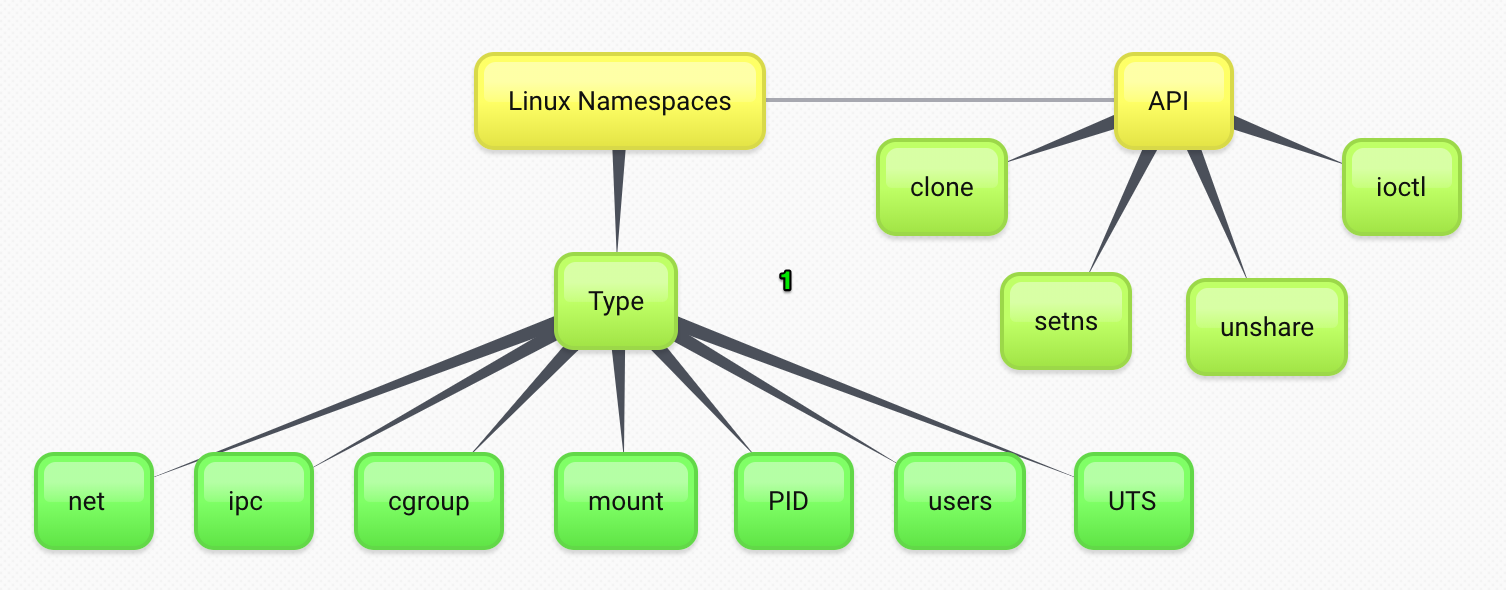
\includegraphics[width=1\textwidth]{img/linux-namespace1.png}
			\caption{Diferentes namespaces en Linux y su API de acceso. (\ref{bib:img1})}
		\end{center}
	\end{figure}
	
	
	\pagebreak
	\subsubsection{Time}
	\par \noindent Por último, nos queda el namespaces asociado al tiempo. Este namespace fue propuesto para que se incorporara al kernel de Linux en 2018 y en enero de 2020 fue añadido a la versión mainline de Linux. Apareció en la release 5.6 del kernel de Linux. \\
	
	\par \noindent El namespace time, permite que por cada namespace que tengamos, podamos crear desfases entre los relojes monotónicos (CLOCK\_MONOTONIC) y de boot (CLOCK\_BOOTTIME), de la máquina host. Esto permite que dentro de los contendores se nos permita cambiar la fecha y la hora, sin tener que modificar la hora del sistema host. Además, supone una capa más de seguridad, ya que no estamos vinculando directamente la hora a los relojes físicos de nuestro sistema.\\
	
	\par \noindent Un namespace de tipo time, es muy similar al namespace de tipo PID en la manera de como lo creamos. Utilizamos el comando unshare -T, y mediante una systemcall se nos creará un nuevo time namespace, pero no lo asocia directamente con el proceso. Tenemos que utilizar setns para asociar un proceso a un namespace, además todos los procesos dependientes también tendrán asignado dicho namespace. 
	
	\addvspace{80px}
	
	\begin{figure}[h]
		\begin{center}
			% https://twitter.com/b0rk/status/1240364585766576128/photo/1
			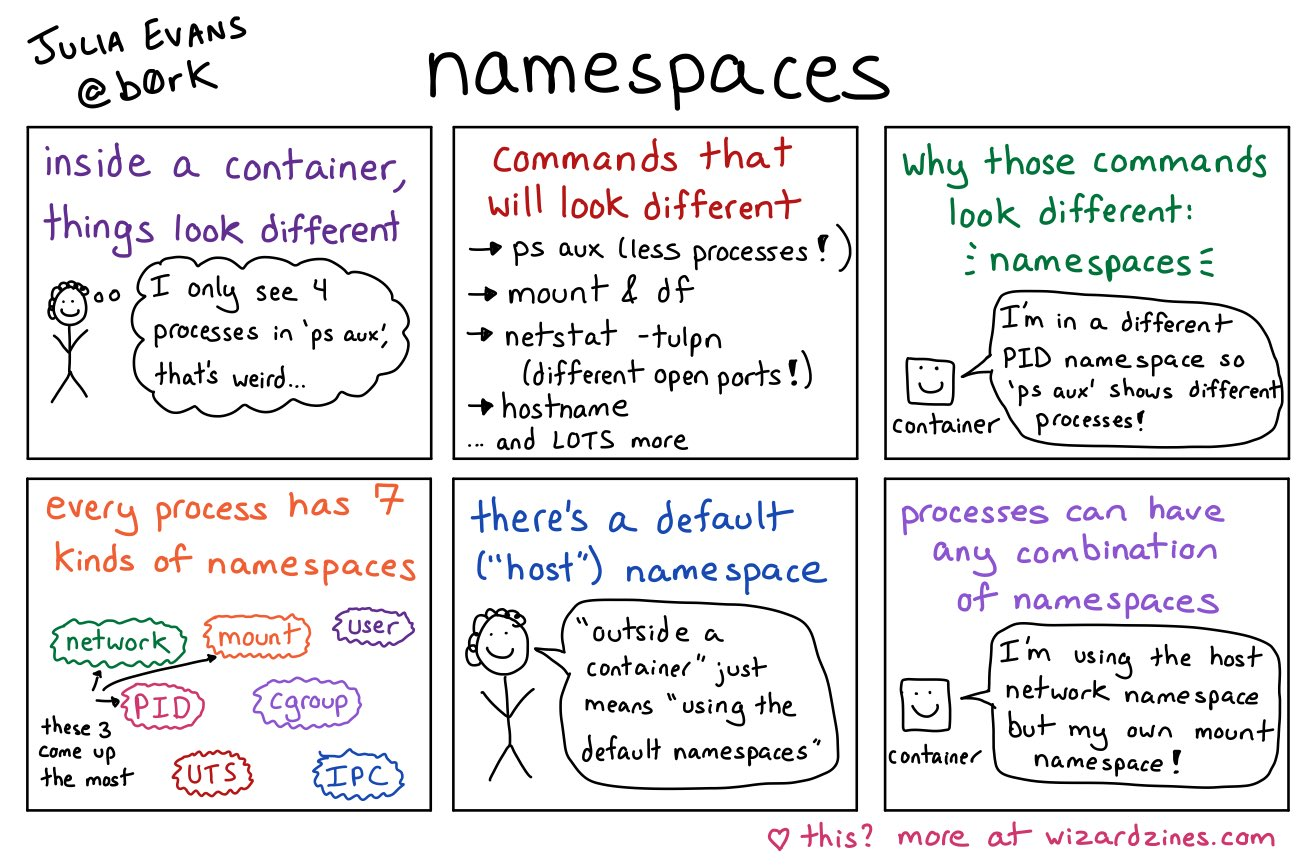
\includegraphics[width=0.8\textwidth]{img/how_containers_work.jpg}
			\caption{Como funcionan los contenedores. (\ref{bib:img2})}
		\end{center}
	\end{figure}
	
	\pagebreak
	
	\subsection{Ejemplo de uso de 'netns' usando comando \texttt{ip}}
	\noindent En este apartado, vamos a detallar un ejemplo de como funciona el comando IP manejando los 'network namespaces'.\\
	
	\noindent Creamos los \textit{network namespaces}, en este caso, con nombre h1 y h2. El sistema no crea directamente el namespace, lo que en realidad hace es definirlos en el sistema. El \textit{network namespace} se crea cuando una aplicación se asocia a el.
	\begin{verbatim}
$ ip netns add h1
$ ip netns add h2
	\end{verbatim}

	\noindent Si utilizamos el comando \texttt{ip netns}, nos mostrará los netns existentes. Como es un sub-comando de \texttt{ip}, muestra los ns que el comando \texttt{lsns} no muestra. \\
	
	\noindent Procedemos a asociar una aplicación a cada netns. Utilizamos \texttt{bash}.
	\begin{verbatim}
$ ip netns exec h1 bash
$ ip netns exec h2 bash
	\end{verbatim}

	\noindent Ahora, si que podemos utilizar el comando \texttt{lsns}. Comprobamos que si nos aparecen los ns que hemos creado, cosa que antes de asociar una aplicación al ns, no pasaba. \\
	
	\noindent El comando \texttt{ip} crea automaticamente un \textit{nsfs} para poder colocar los archivos de configuración del \textit{netns}. Para ello, debe crearse el directorio \texttt{/etc/netns/h1} y poner en el los archivos de configuración de la red.
	\begin{verbatim}
$ mkdir /etc/netns/h1
$ echo "nameserver 8.8.8.8" > /etc/netns/h1/resolv.conf
	\end{verbatim}

	\noindent En este momento, tenemos el ns configurado con DNS. Nos quedaría realizar la conexión entre el ethernet físico de nuestro \textit{host} y las interfaces de nuestros namespaces. Para ello, vamos a utilizar un conmutador virtual, en este caso Open vSwitch.
	\begin{verbatim}
$ systemctl enable --now openvswitch.service
	\end{verbatim}

	\noindent Creamos un \textit{brige} utilizando el OpenvSwitch.
	\begin{verbatim}
$ $ ovs-vsctl add-br s1
	\end{verbatim}

	\noindent Utilizando el comando \texttt{ip}, creamos las interfaces virtuales de ethernet y las asignamos a sus namespaces.
	\begin{verbatim}
$ ip link add h1-eth0 type veth peer name s1-eth1
$ ip link add h2-eth0 type veth peer name s1-eth2
$ ip link set h1-eth0 netns h1
$ ip link set h2-eth0 netns h2
	\end{verbatim}

	\pagebreak
	
	\noindent Utilizando el comando \texttt{ovs-vsctl}, asignamos al \textit{bridge} el otro par ethernet que hemos creado para cada namespace.
	\begin{verbatim}
$ ovs-vsctl add-port s1 s1-eth1
$ ovs-vsctl add-port s1 s1-eth2
	\end{verbatim}

	\noindent Verificamos que el controlador sea \textit{standalone}, así el switch se comportará como un \textit{learning-switch}.
	\begin{verbatim}
$ ovs-vsctl set-fail-mode br0 standalone
	\end{verbatim}

	\noindent Como la conexión es desde localhost al exterior, entendemos que es una conexión fuera de banda.
	\begin{verbatim}
$ ovs-vsctl set controller br0 connection-mode=out-of-band
	\end{verbatim}

	\noindent En este momento, tenemos todos configurado a falta de habilitar las diferentes interfaces de nuestra topología.
	\begin{verbatim}
$ ip netns exec h1 ip link set h1-eth0 up
$ ip netns exec h1 ip link set lo up
$ ip netns exec h1 ip add add 10.0.0.1/24 dev h1-eth0
$ ip netns exec h2 ip link set h2-eth0 up
$ ip netns exec h2 ip link set lo up
$ ip netns exec h2 ip add add 10.0.0.2/24 dev h2-eth0
$ ip link set s1-eth1 up
$ ip link set s1-eth2 up
	\end{verbatim}

	\noindent Ahora tenemos todas las interfaces configuradas, el switch activado y el sistema interconectado, por lo que podemos ejecutar un ping en una de las terminales de los namespaces para verificar la topología.
	\begin{verbatim}
$ ip netns exec h1 ping -c4 10.0.0.2
	\end{verbatim}

	\noindent Si queremos revertir todas las configuraciones que hemos hecho, lo que tenemos que hacer es ejecutar los siguientes comandos:
	\begin{verbatim}
$ ovs-vsctl del-br s1
$ ip link delete s1-eth1
$ ip link delete s1-eth2
$ ip netns del h1
$ ip netns del h2
	\end{verbatim}

	\pagebreak

	\subsection{Ejemplo de uso de 'netns' usando comando \texttt{unshare}}
	\noindent En el ejemplo anterior, utilizabamos el comando \texttt{ip} para manejar los netns, sin embargo, eso nos limitaba los tipos namespaces que queriamos asignar a nuestro namespace. En contra partida a esto, el comando \texttt{unshare} nos da más libertad a la hora de crear los namespaces. \\
	
	\noindent Utilizando \texttt{unshare}, no podemos ponerle un nombre, pero sí que nos permite asociarlo a un archivo, que montará con tipo bind. Esto nos permitirá utilizar en namespace aunque no haya ningún proceso corriendo en el, para ello podemos utilizar el comando \texttt{nsenter}.
	\begin{verbatim}
$ touch /var/net-h1
$ touch /var/uts-h1
$ unshare --net=/var/net-h1 --uts=/var/uts-h1 /bin/bash
	\end{verbatim}

	\noindent Utilizando el comando \texttt{nsenter} podemos ejecutar comandos dentro del namespace.
	\begin{verbatim}
$ nsenter --net=/var/net-h1 --uts=/var/uts-h1 hostname h1
$ nsenter --net=/var/net-h1 --uts=/var/uts-h1 ip address
	\end{verbatim}

	\noindent Para destruir el namespace, lo que tendremos que hacer es desmontar los archivos asignados a dicho namespace.
	\begin{verbatim}
$ umount /var/net-h1
$ umount /var/uts-h1
	\end{verbatim}

	\noindent Como será común necesitar más de un namespace, de ahora en adelante tendremos que utilizar los comandos \texttt{unshare} y \texttt{nsenter}.

	\pagebreak
	
	\section{Virtualización}
	\subsection{Contenedores usando \texttt{unshare}}
	\subsection{Contenedores LXC}
	\subsection{Contenedores Docker}
	
	\pagebreak

	\section{Caso práctico: Virtualización para simulación de redes}
	\subsection{Evaluación de prestaciones}
	\subsection{Interconexión física de diferentes red virtuales}
	\subsection{Openflow OKO}
	
	\pagebreak
	
	\section{Conclusiones}

	%%% Bibliography
	\pagebreak
	\section*{Bibliografía}
	\addcontentsline{toc}{section}{Bibliografía}
	\subsection*{Enlaces y referencias}
	\addcontentsline{toc}{subsection}{Enlaces y referencias}
	%%\hyperref[bib:link1]{\emph{Reference of bibliography}}
	\begin{enumerate}
		%1
		\item 
		\label{bib:link1} \href{https://lwn.net/Articles/531114/}{\textit{Namespaces}}
		
		%2
		\item 
		\label{bib:link2} \href{https://laurel.datsi.fi.upm.es/~ssoo/SOA/namespaces.html}{Tutorial: Espacio de nombres en Linux}
		
		%3
		\item 
		\label{bib:link3} \href{https://www.phoronix.com/scan.php?page=news_item&px=Linux-Time-Namespace-Coming}{\textit{Time namespaces coming to linux}}
		
		%4
		\item 
		\label{bib:link4} \href{https://platform.sh/blog/2020/the-container-is-a-lie/}{\textit{Container is a lie. Namespaces}}
		
		%5
		\item 
		\label{bib:link5} \href{https://locurastecnicas.blogspot.com/2020/09/linux-namespaces-y-cgroups.html}{\textit{Namespaces.} Uso de \textit{cgroups}.}
		
		%6
		\item 
		\label{bib:link6} \href{https://www.youtube.com/watch?v=_WgUwUf1d34}{\textit{Introduction to Network Namespaces}}
		
		
		%7
		\item
		\label{bib:link7} \href{https://www.redhat.com/sysadmin/mount-namespaces}{\textit{Build a container by hand: the mount namespace}}
		
		
		%8
		\item
		\label{bib:link8}
		\href{https://en.wikipedia.org/wiki/Process_identifier}{Indentificador de procesos (\textit{process id})}
		
		
		%9
		\item
		\label{bib:link9}
		\href{https://www.redhat.com/sysadmin/linux-pid-namespaces}{\textit{Linux PID namespaces work with containers}}
		
		%10
		\item
		\label{bib:link10}
		\href{https://blogs.igalia.com/dpino/2016/04/10/network-namespaces/}{\textit{Network Namespaces}}
		
		%11
		\item
		\label{bib:link11}
		\href{https://developers.redhat.com/blog/2018/10/22/introduction-to-linux-interfaces-for-virtual-networking#veth}{\textit{Introduction to Linux interfaces for virtual networking}}
		
		
		%12
		\item
		\label{bib:link12}
		\href{https://elpuig.xeill.net/Members/vcarceler/articulos/introduccion-a-los-grupos-de-control-cgroups-de-linux}{\textit{Introducción a los grupos de control (cgroups) de Linux}}
		
		%13
		\item
		\label{bib:link13}
		\href{https://git.kernel.org/pub/scm/linux/kernel/git/tip/tip.git/commit/?h=timers/core&id=769071ac9f20b6a447410c7eaa55d1a5233ef40c}{\textit{Time namespaces}}
		
		%14
		\item
		\label{bib:link14}
		\href{https://blog.scottlowe.org/2013/09/04/introducing-linux-network-namespaces/}{\textit{Network namespaces. Assign and configure}}
		
		
		%15
		\item
		\label{bib:configure host-only}
		\href{https://www.tecmint.com/network-between-guest-vm-and-host-virtualbox/}{How to configure Network Between Guest VM and Host in Virtualbox}
		
		
		%16
		\item
		\label{bib:install ansible}
		\href{https://www.cyberciti.biz/faq/how-to-install-ansible-on-fedora-for-it-and-server-automation/}{How to install ansible on fedora for it and server automation}
		
		%17
		\item
		\label{bib: herramientas virtualizacion}
		\href{https://www.uv.es/sto/charlas/2010_CIM/hvl-cim-2010.html/index.html}{\textit{Herramientas de virtualización libres para sistemas GNU/Linux}}
		
		%18
		\item
		\label{paper nfv 2012}
		\href{https://portal.etsi.org/nfv/nfv_white_paper.pdf}{NFV white paper}
		
		%19
		\item
		\label{youtube: nfv y sdn cristina}
		\href{https://www.youtube.com/watch?v=3JEAK66wujg}{Youtube: NFV y SDN: las redes del futuro y del presente - Cristina Santana | T3chFest 2018}
		
		%20
		\item
		\label{servers running linux}
		\href{https://hostingtribunal.com/blog/linux-statistics/}{Percentage of server that run in Linux}
		
		% X
		\item
		\label{bib:link20}
		\href{https://jsitech1.gitbooks.io/meet-docker/content/fundamentos_de_docker.html}{Fundamentos de Docker}
		
	\end{enumerate}

	\pagebreak

	\subsection*{Imágenes}
	\addcontentsline{toc}{subsection}{Imagenes}
	\begin{enumerate}
		%1
		\item 
		\label{bib:img1}\href{https://8gwifi.org/docs/linux-namespace.jsp}{Namespaces y API de acceso.}
		
		%2
		\item 
		\label{bib:img2}\href{https://twitter.com/b0rk/status/1240364585766576128}{How containers work.}
		
		
	\end{enumerate}

	\pagebreak
	
	\pagebreak
	\section*{Anexos}
	\addcontentsline{toc}{section}{Anexos}
	\subsection*{Anexo 1. Instalación de \texttt{ansible} para automatizar una VM}
	\addcontentsline{toc}{subsection}{Anexo 1. Instalación \texttt{ansible}}
	\noindent En el caso de que queramos utilizar la herramienta ansible para configurar una VM, tendremos que seguir los siguientes pasos.
	\begin{enumerate}
		\item Asegurarnos de que tenemos instalado el programa en el host. La principal dependencia de \texttt{ansible} es \texttt{Python}. \\
		Para instalar \texttt{ansible} en diferentes distribuciones sería tal que:
		\begin{itemize}
			\item Ubuntu 21.04:
			\begin{verbatim}
				$ sudo apt install -y software-properties-common
				$ sudo add-apt-repository --yes --update ppa:ansible/ansible
				$ sudo apt update
				$ sudo apt install -y ansible
			\end{verbatim}
			
			\item Fedora 32:
			\begin{verbatim}
				$ sudo dnf update
				$ sudo dnf install ansible
			\end{verbatim}
			
			\item OpenSUSE:
			\begin{verbatim}
				$ zypper in ansible
			\end{verbatim}
			
			\item Arch Linux:
			\begin{verbatim}
				$ sudo pacman -S ansible
			\end{verbatim} 
		\end{itemize}
		
		\item Creamos una clave SSH para utilizarla como método de autentificación con la maquina virtual. 
		\begin{verbatim}
			(host)$ ssh-keygen -t ed25519 -C "Host Ansible ssh key"
		\end{verbatim}
		
		\item Utilizando nuestro gestor de máquinas virtuales, encendemos la VM. Es importante que nos aseguremos que tiene internet, por lo que configuramos que la interfaz de red sea de tipo \textit{NAT}. Dentro de la máquina, buscaremos que ip tiene asignada con el comando \texttt{ip address}. Desde este momento, dejaremos la máquina virtual encendida.
		
		\item Procedemos a copiar la clave pública SSH que hemos generado en el paso dos. Utilizamos el siguiente comando, sustituyendo con el usuario e IP específico de la máquina. Tendremos que configurar una red tipo \textit{Host-only network} para poder comunicarnos correctamente con nuestra máquina virtual, para ello podemos seguir los pasos detallados en [\ref{bib:configure host-only}]
		\begin{verbatim}
			(host)$ ssh-copy-id -i $HOME/.ssh/id_ed25519.pub <user>@<IP VM>
		\end{verbatim}
		
		\pagebreak
		
		\item En este momento ya podríamos conectar con la máquina virtual utilizando \texttt{ansible}. Sin embargo, por comodidad, lo que vamos a hacer es crear un archivo que funcione con inventario de servidores. Nos servirá para guardar las direcciones IP de los servidores en los que queremos ejecutar comandos remotos con \texttt{ansible}. Para ello, creamos un archivo \texttt{inventory}. Como ejemplo, dicho archivo puede ser tal que:
		\begin{verbatim}
			## VMs locals 
			[virtualbox]
			10.0.100.1
			10.0.100.2
			
			## Server SSH
			[server]
			192.168.1.200
		\end{verbatim}
		
		\item Para probar la conectividad. Nos aseguramos de que tenemos la máquina virtual encendida y que además, hemos copiado la clave ssh y tenemos su IP añadida a nuestro inventario. Después, procedemos a ejecutar el siguiente comando en la máquina host:
		\begin{verbatim}
			(host)$ ansible -i inventory -m ping
		\end{verbatim}
		\noindent En la consola nos aparecerá la información de cada uno de las IP que habrá probado para ejecutar el comando remoto \texttt{ping}.
	\end{enumerate}
	
	\pagebreak
	
	\subsection*{Anexo 2. Configuración de \textit{Guest Network} para comunicar con la VM}
	\addcontentsline{toc}{subsection}{Anexo 2. Configuración de \textit{Guest Network} para comunicar con la VM}
	\noindent Para comunicar nuestra máquina host [\ref{bib:configure host-only}], con una \textit{virtual machine} es necesario que estén en una misma red, es por esto por lo que vamos a crear una red en especifico para ello. En el programa \textit{Virtualbox}, esta funcionalidad recibe el nombre de \textit{Host-only}.\\
	
	\noindent Es importante que cuando queramos configurar una máquina virtual con esta funcionalidad que siempre pongamos el adaptador de red 1 como el que tendrá la comunicación \textit{guest}, mientras que el adaptador 2 será el que tendrá la conexión a internet via \textit{NAT}.\\
	
	\noindent Procedemos a enumerar los pasos a seguir para configurar una máquina virtual con conectividad con el host, utilizando \textit{Virtualbox}.
	
	\begin{enumerate}
		\item Abrimos el programa \textit{Virtualbox}. Navegamos a la sección: \textbf{File $\rightarrow$ Preferences}.
		\item Seleccionamos la tabla de \textbf{\textit{Host-only Networks}}. Procedemos a pulsar el botón + para añadir una nueva red.
		\item Asignamos las diferentes IP que considermos. Es importante que dejemos activado el servidor DHCP, así la máquina virtual tendrá una IP válida dentro de la red.
		\item Ahora, lo que tenemos que hacer es añadir una interfaz de red a nuestra máquina virtual. Para ello, vamos a las \textbf{Setting}s de la máquina virtual. En el apartado de Network, cambiamos el \textbf{Adapter 1} a\textbf{ Host-only Adapter}, y asignamos una segunda interfaz de red con NAT (Adapter 2 attached to NAT).
		\item Para comprobar que lo hemos hecho correctamente. Arrancamos la máquina virtual, ejecutamos el comando \texttt{ip address}. Nos deberían aparacer las diferentes interfaces que previamente hemos configurado, es decir, una interfaz de loopback, otra que corresponde al Host-only network, y por último, una que corresponda con la interfaz de NAT.
	\end{enumerate}
	
	\pagebreak
	\subsection*{Anexo 3. Playbooks \texttt{ansible}}
	\addcontentsline{toc}{subsection}{Anexo 3. Playbooks \texttt{ansible}}
\end{document}